\documentclass{article}
\usepackage[utf8]{inputenc}
\usepackage{graphicx}
\usepackage{hyperref}

\usepackage{array}
\usepackage{multirow}

\newcommand\MyBox[2]{
  \fbox{\lower0.75cm
    \vbox to 1.7cm{\vfil
      \hbox to 1.7cm{\hfil\parbox{1.4cm}{#1\\#2}\hfil}
      \vfil}%
  }%
}

\title{CSI 5387 Data Mining and Concept Learning Assignment 2}
\author{Lingfeng Zhang 300134245}
\date{February 2020}

\begin{document}

\maketitle

In this assignment, I used Python to handle it.

GitHub Source Code: \href{https://github.com/RichardChangCA/CSI-5387-Data-Mining-and-Concept-Learning/tree/master/Assignment_2}{https://github.com/RichardChangCA/CSI-5387-Data-Mining-and-Concept-Learning/tree/master/Assignment\_2}

\section{A. Data Preprocessing}

\subsection{1.}

About the missing value, I used sklearn.inpute.SimpleImputer to impute the missing value. For the strategy attribute, I chose the most frequent value, which means the mode value for each attributes, to impute.

Central measure of tendency used in handling missing data: mode value

\subsection{2.}

Neural network can perform well when the input data are scaled in the same range because some attribute values will be dominant without scaling.

In this assignment, I used sklearn.preprocessing.MinMaxScalar to scale the input data.

Method of re-scaling the data with a normalizing: min-max normalization

\section{B. Model Development}

\subsection{Single Layer}

\subsubsection{1.}

In this section, I used TensorFlow version 2.0 deep learning framework combined with Keras to build up neural network models. Dense layers in Keras represent fully-connected layers. 

In the single node model, there are 1 unit in the dense layer,which output dimension is 1 value and input dimension is 8, because it is a binary classification task and meaningful attributes have 8 columns.

There are several hyper-parameters I set:

bias usage: True

activation function: Sigmoid

Optimizer: SGD(Stochastic gradient descent)

learning rate: 0.01

Loss function: binary cross-entropy

Training epoch: 100

The loss plot is shown below, and decreasing loss value means the model is learning.

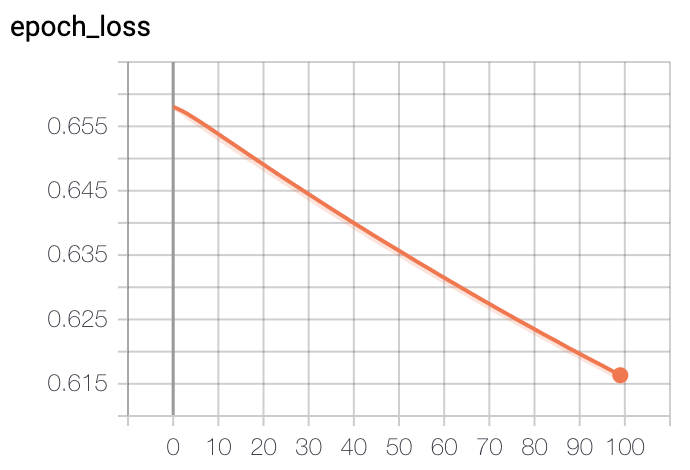
\includegraphics[scale=0.5]{single_layer_loss.png}

\subsubsection{2.}

The neural network plot is shown below.

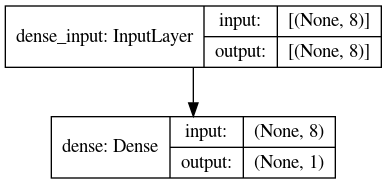
\includegraphics[scale=0.5]{single_layer_model.png}

There are 9 parameters in total, where 8 parameters are weights and 1 parameter is the bias.

\subsubsection{3. Model Performance}

accuracy: 0.59375

some predictions:

1. X=[[0.11764706 0.39354839 0.6557377  0.41304348 0.22576832 0.31697342
  0.27028181 0.13333333]], prediction=[[0]], actual=1

2. X=[[0.29411765 0.41935484 0.50819672 0.36956522 0.15248227 0.3599182
  0.18616567 0.06666667]], prediction=[[0]], actual=1

3. X=[[0.23529412 0.70967742 0.59016393 0.23913043 0.14893617 0.26789366
  0.11101623 0.26666667]], prediction=[[0]], actual=0

4. X=[[0.35294118 0.39354839 0.57377049 0.27173913 0.08037825 0.25766871
  0.01878736 0.26666667]], prediction=[[0]], actual=0

5. X=[[0.70588235 0.36129032 0.68852459 0.2826087  0.12411348 0.24130879
  0.17506405 0.41666667]], prediction=[[0]], actual=0



\subsubsection{4. Confusion Matrix}

\noindent
\renewcommand\arraystretch{1.5}
\setlength\tabcolsep{0pt}
\begin{tabular}{c >{\bfseries}r @{\hspace{0.7em}}c @{\hspace{0.4em}}c @{\hspace{0.7em}}l}
  \multirow{10}{*}{\parbox{1.1cm}{\bfseries\raggedleft Actual\\ value}} & 
    & \multicolumn{2}{c}{\bfseries Prediction outcome} & \\
  & & \bfseries p & \bfseries n & \bfseries total \\
  & p$'$ & \MyBox{0}{} & \MyBox{78}{} & 78 \\[2.4em]
  & n$'$ & \MyBox{0}{} & \MyBox{114}{} & 114 \\
  & total & 0 & 192 &
\end{tabular}

sensitivity:0.0

specificity:1.0

\subsection{Multi-Layer}

\subsubsection{1.}

The image below is the structure of multi-layer perceptron, which has 5 hidden nodes and 2 hidden layers. In this case, I maintained the same hyper-parameter as the single node perceptron.

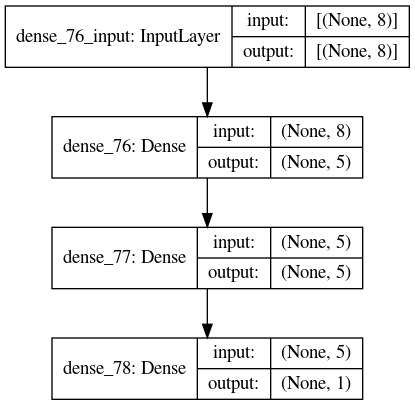
\includegraphics[scale=0.5]{multilayer_True_sigmoid_0.01_100.png}

The accuracy is also 0.59375 because the model predicts all tuples are negative. Both single node perceptron and multi-layer perceptron fail to perform well without fine-tuning.

The loss plot is shown below.

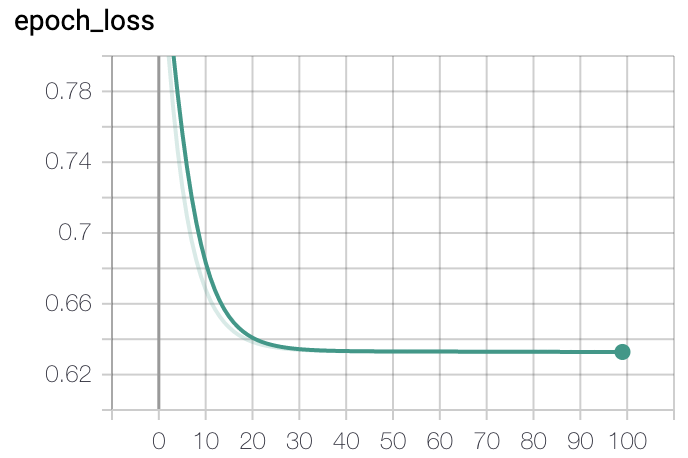
\includegraphics[scale=0.5]{multi_layer_loss.png}

\subsubsection{2.}

Activation function, learning rate, training epochs and bias existence are hyper-parameter we can fine-tune.

In this assignment, I chose several values for these hyper-parameters and get various results.

Activation function: sigmoid, relu, tanh

Learning rate: 0.1, 0.01, 0.001

Training epochs: 50, 100, 200

Bias existence: True, False

The results are shown in the appendix.

The loss plot of the multi-layer perceptron with the highest accuracy in shown in below.

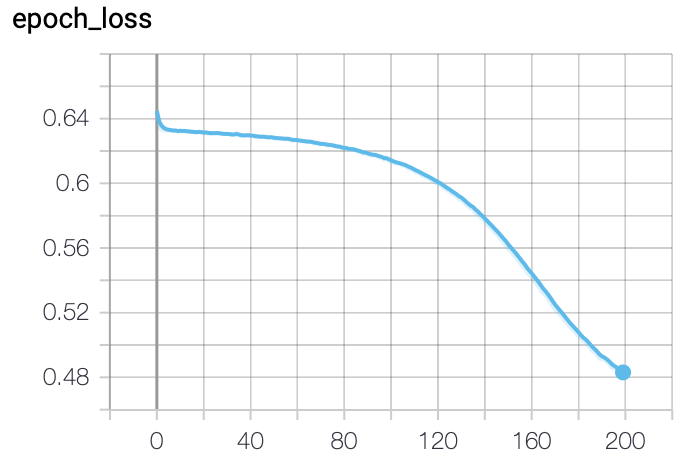
\includegraphics[scale=0.5]{best_multi_layer_loss.png}

The hyper-parameters of the highest accuracy multi-layer perceptron are:

Activation function: sigmoid

Learning rate: 0.1

Training epochs: 200

Bias existence: True

\subsection{C. Model Comparison}

SVM results are shown below:

accuracy:0.7552083333333334

TP:35

TN:110

FP:4

FN:43

sensitivity:0.44871794871794873

specificity:0.9649122807017544

\subsection{D. Model Evaluation}

\subsubsection{1.}

Multi-layer perceptron:

accuracy:0.59375

sensitivity:0.0

specificity:1.0

\bigskip

Multi-layer perceptron with fine-tuning:

accuracy:0.7552083333333334

sensitivity:0.47435897435897434

specificity:0.9473684210526315

\bigskip

SVM:

accuracy:0.7552083333333334

sensitivity:0.44871794871794873

specificity:0.9649122807017544

\subsubsection{2.}

1.In the case of multi-layer perceptron without fine-tuning:

SVM performs best and multi-layer perceptron performs worst in criteria of accuracy and sensitivity.

Multi-layer perceptron performs best and SVM performs worst in criteria of specificity.

\bigskip

2.In the case of multi-layer perceptron with fine-tuning:

SVM performs same as multi-layer perceptron in criteria of accuracy

SVM performs best and multi-layer perceptron performs worst in criteria of specificity.

Multi-layer perceptron performs best and SVM performs worst in criteria of sensitivity.

In conclusion, various hyper-parameter combinations in multi-layer perceptron performs different.

\subsubsection{3.}

ROC curve is shown in below.

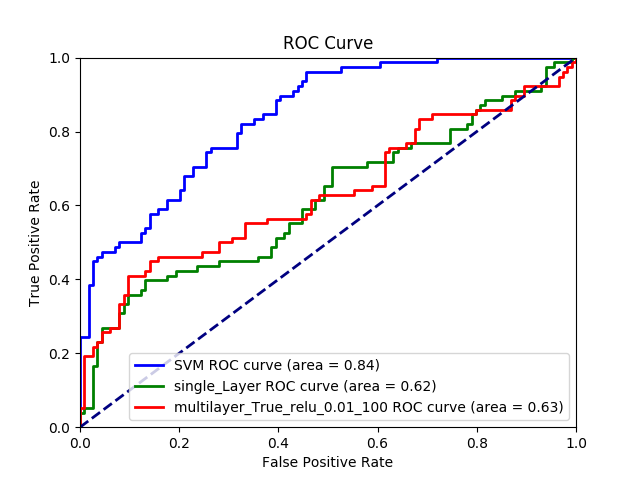
\includegraphics[scale=0.5]{roc_curve.png}

SVM performs better than single node and multi-layer perceptron because AUC of SVM is greater than others.

ROC curve of fine-tuned multi-layer perceptron and SVM is shown in below and SVM is also the best model.

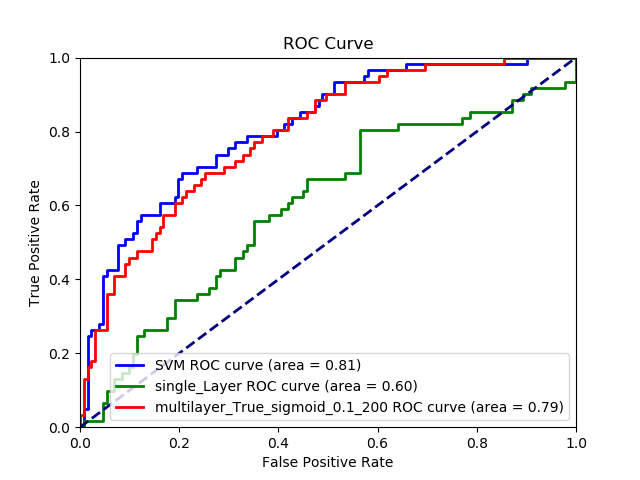
\includegraphics[scale=0.5]{roc_curve_fine_tune.png}

\subsection{Appendix}

\subsection{bias: False, activation: tanh, lr: 0.001, epochs: 50}

TP:2

TN:114

FP:0

FN:76

accuracy:0.6041666666666666

sensitivity:0.02564102564102564

specificity:1.0



\subsection{bias: True, activation: sigmoid, lr: 0.0001, epochs: 50}

TP:0

TN:114

FP:0

FN:78

accuracy:0.59375

sensitivity:0.0

specificity:1.0



\subsection{bias: False, activation: relu, lr: 0.01, epochs: 50}

TP:0

TN:114

FP:0

FN:78

accuracy:0.59375

sensitivity:0.0

specificity:1.0



\subsection{bias: True, activation: relu, lr: 0.0001, epochs: 50}

TP:2

TN:113

FP:1

FN:76

accuracy:0.5989583333333334

sensitivity:0.02564102564102564

specificity:0.9912280701754386



\subsection{bias: False, activation: relu, lr: 0.0001, epochs: 100}

TP:21

TN:105

FP:9

FN:57

accuracy:0.65625

sensitivity:0.2692307692307692

specificity:0.9210526315789473



\subsection{bias: False, activation: tanh, lr: 0.0001, epochs: 100}

TP:0

TN:114

FP:0

FN:78

accuracy:0.59375

sensitivity:0.0

specificity:1.0



\subsection{bias: True, activation: tanh, lr: 0.01, epochs: 200}

TP:40

TN:100

FP:14

FN:38

accuracy:0.7291666666666666

sensitivity:0.5128205128205128

specificity:0.8771929824561403



\subsection{bias: True, activation: tanh, lr: 0.001, epochs: 50}

TP:14

TN:111

FP:3

FN:64

accuracy:0.6510416666666666

sensitivity:0.1794871794871795

specificity:0.9736842105263158



\subsection{bias: True, activation: relu, lr: 0.0001, epochs: 200}

TP:0

TN:114

FP:0

FN:78

accuracy:0.59375

sensitivity:0.0

specificity:1.0



\subsection{bias: True, activation: relu, lr: 0.001, epochs: 100}

TP:0

TN:114

FP:0

FN:78

accuracy:0.59375

sensitivity:0.0

specificity:1.0



\subsection{bias: False, activation: relu, lr: 0.001, epochs: 200}

TP:21

TN:111

FP:3

FN:57

accuracy:0.6875

sensitivity:0.2692307692307692

specificity:0.9736842105263158



\subsection{bias: False, activation: sigmoid, lr: 0.0001, epochs: 200}

TP:0

TN:114

FP:0

FN:78

accuracy:0.59375

sensitivity:0.0

specificity:1.0



\subsection{bias: False, activation: tanh, lr: 0.01, epochs: 200}

TP:42

TN:102

FP:12

FN:36

accuracy:0.75

sensitivity:0.5384615384615384

specificity:0.8947368421052632



\subsection{bias: False, activation: sigmoid, lr: 0.001, epochs: 200}

TP:0

TN:114

FP:0

FN:78

accuracy:0.59375

sensitivity:0.0

specificity:1.0



\subsection{bias: False, activation: sigmoid, lr: 0.0001, epochs: 50}

TP:78

TN:0

FP:114

FN:0

accuracy:0.40625

sensitivity:1.0

specificity:0.0



\subsection{bias: True, activation: sigmoid, lr: 0.001, epochs: 100}

TP:0

TN:114

FP:0

FN:78

accuracy:0.59375

sensitivity:0.0

specificity:1.0



\subsection{bias: False, activation: tanh, lr: 0.01, epochs: 50}

TP:38

TN:106

FP:8

FN:40

accuracy:0.75

sensitivity:0.48717948717948717

specificity:0.9298245614035088



\subsection{bias: True, activation: sigmoid, lr: 0.001, epochs: 200}

TP:0

TN:114

FP:0

FN:78

accuracy:0.59375

sensitivity:0.0

specificity:1.0



\subsection{bias: False, activation: tanh, lr: 0.01, epochs: 100}

TP:38

TN:104

FP:10

FN:40

accuracy:0.7395833333333334

sensitivity:0.48717948717948717

specificity:0.9122807017543859



\subsection{bias: False, activation: tanh, lr: 0.001, epochs: 200}

TP:33

TN:107

FP:7

FN:45

accuracy:0.7291666666666666

sensitivity:0.4230769230769231

specificity:0.9385964912280702



\subsection{bias: False, activation: tanh, lr: 0.0001, epochs: 200}

TP:1

TN:113

FP:1

FN:77

accuracy:0.59375

sensitivity:0.01282051282051282

specificity:0.9912280701754386



\subsection{bias: True, activation: sigmoid, lr: 0.0001, epochs: 200}

TP:0

TN:114

FP:0

FN:78

accuracy:0.59375

sensitivity:0.0

specificity:1.0



\subsection{bias: True, activation: sigmoid, lr: 0.01, epochs: 50}

TP:0

TN:114

FP:0

FN:78

accuracy:0.59375

sensitivity:0.0

specificity:1.0



\subsection{bias: False, activation: relu, lr: 0.001, epochs: 50}

TP:0

TN:114

FP:0

FN:78

accuracy:0.59375

sensitivity:0.0

specificity:1.0



\subsection{bias: False, activation: relu, lr: 0.0001, epochs: 200}

TP:5

TN:110

FP:4

FN:73

accuracy:0.5989583333333334

sensitivity:0.0641025641025641

specificity:0.9649122807017544



\subsection{bias: True, activation: tanh, lr: 0.001, epochs: 200}

TP:41

TN:103

FP:11

FN:37

accuracy:0.75

sensitivity:0.5256410256410257

specificity:0.9035087719298246



\subsection{bias: True, activation: tanh, lr: 0.0001, epochs: 100}

TP:4

TN:112

FP:2

FN:74

accuracy:0.6041666666666666

sensitivity:0.05128205128205128

specificity:0.9824561403508771



\subsection{bias: False, activation: sigmoid, lr: 0.001, epochs: 100}

TP:0

TN:114

FP:0

FN:78

accuracy:0.59375

sensitivity:0.0

specificity:1.0



\subsection{bias: True, activation: relu, lr: 0.0001, epochs: 100}

TP:0

TN:114

FP:0

FN:78

accuracy:0.59375

sensitivity:0.0

specificity:1.0



\subsection{bias: False, activation: tanh, lr: 0.0001, epochs: 50}

TP:0

TN:113

FP:1

FN:78

accuracy:0.5885416666666666

sensitivity:0.0

specificity:0.9912280701754386



\subsection{bias: False, activation: tanh, lr: 0.001, epochs: 100}

TP:7

TN:114

FP:0

FN:71

accuracy:0.6302083333333334

sensitivity:0.08974358974358974

specificity:1.0



\subsection{bias: False, activation: sigmoid, lr: 0.01, epochs: 50}

TP:0

TN:114

FP:0

FN:78

accuracy:0.59375

sensitivity:0.0

specificity:1.0



\subsection{bias: False, activation: sigmoid, lr: 0.001, epochs: 50}

TP:0

TN:114

FP:0

FN:78

accuracy:0.59375

sensitivity:0.0

specificity:1.0



\subsection{bias: True, activation: relu, lr: 0.001, epochs: 200}

TP:35

TN:109

FP:5

FN:43

accuracy:0.75

sensitivity:0.44871794871794873

specificity:0.956140350877193



\subsection{bias: True, activation: tanh, lr: 0.0001, epochs: 50}

TP:0

TN:114

FP:0

FN:78

accuracy:0.59375

sensitivity:0.0

specificity:1.0



\subsection{bias: False, activation: relu, lr: 0.0001, epochs: 50}

TP:0

TN:114

FP:0

FN:78

accuracy:0.59375

sensitivity:0.0

specificity:1.0



\subsection{bias: True, activation: relu, lr: 0.001, epochs: 50}

TP:0

TN:114

FP:0

FN:78

accuracy:0.59375

sensitivity:0.0

specificity:1.0



\subsection{bias: False, activation: relu, lr: 0.01, epochs: 100}

TP:59

TN:82

FP:32

FN:19

accuracy:0.734375

sensitivity:0.7564102564102564

specificity:0.7192982456140351



\subsection{bias: True, activation: tanh, lr: 0.0001, epochs: 200}

TP:0

TN:114

FP:0

FN:78

accuracy:0.59375

sensitivity:0.0

specificity:1.0



\subsection{bias: True, activation: relu, lr: 0.01, epochs: 200}

TP:45

TN:99

FP:15

FN:33

accuracy:0.75

sensitivity:0.5769230769230769

specificity:0.868421052631579



\subsection{bias: False, activation: sigmoid, lr: 0.0001, epochs: 100}

TP:0

TN:114

FP:0

FN:78

accuracy:0.59375

sensitivity:0.0

specificity:1.0



\subsection{bias: False, activation: sigmoid, lr: 0.01, epochs: 100}

TP:0

TN:114

FP:0

FN:78

accuracy:0.59375

sensitivity:0.0

specificity:1.0



\subsection{bias: False, activation: sigmoid, lr: 0.01, epochs: 200}

TP:20

TN:113

FP:1

FN:58

accuracy:0.6927083333333334

sensitivity:0.2564102564102564

specificity:0.9912280701754386



\subsection{bias: True, activation: tanh, lr: 0.01, epochs: 50}

TP:38

TN:103

FP:11

FN:40

accuracy:0.734375

sensitivity:0.48717948717948717

specificity:0.9035087719298246



\subsection{bias: True, activation: relu, lr: 0.01, epochs: 100}

TP:34

TN:106

FP:8

FN:44

accuracy:0.7291666666666666

sensitivity:0.4358974358974359

specificity:0.9298245614035088



\subsection{bias: True, activation: relu, lr: 0.01, epochs: 50}

TP:39

TN:101

FP:13

FN:39

accuracy:0.7291666666666666

sensitivity:0.5

specificity:0.8859649122807017



\subsection{bias: True, activation: sigmoid, lr: 0.001, epochs: 50}

TP:0

TN:114

FP:0

FN:78

accuracy:0.59375

sensitivity:0.0

specificity:1.0



\subsection{bias: True, activation: tanh, lr: 0.001, epochs: 100}

TP:0

TN:114

FP:0

FN:78

accuracy:0.59375

sensitivity:0.0

specificity:1.0



\subsection{bias: True, activation: sigmoid, lr: 0.01, epochs: 100}

TP:0

TN:114

FP:0

FN:78

accuracy:0.59375

sensitivity:0.0

specificity:1.0



\subsection{bias: True, activation: sigmoid, lr: 0.01, epochs: 200}

TP:37

TN:108

FP:6

FN:41

accuracy:0.7552083333333334

sensitivity:0.47435897435897434

specificity:0.9473684210526315



\subsection{bias: True, activation: tanh, lr: 0.01, epochs: 100}

TP:39

TN:100

FP:14

FN:39

accuracy:0.7239583333333334

sensitivity:0.5

specificity:0.8771929824561403



\subsection{bias: False, activation: relu, lr: 0.001, epochs: 100}

TP:0

TN:114

FP:0

FN:78

accuracy:0.59375

sensitivity:0.0

specificity:1.0



\subsection{bias: True, activation: sigmoid, lr: 0.0001, epochs: 100}

TP:0

TN:114

FP:0

FN:78

accuracy:0.59375

sensitivity:0.0

specificity:1.0



\subsection{bias: False, activation: relu, lr: 0.01, epochs: 200}

TP:37

TN:103

FP:11

FN:41

accuracy:0.7291666666666666

sensitivity:0.47435897435897434

specificity:0.9035087719298246

\end{document}